\chapter{Мировые листы, поворот Вика и дуальность каналов}

\lectureoverview{Частица прочерчивает мировую линию; струна заметает мировой лист. Квантование любого из этих объектов требует суммирования по историям, но лоренцева сумма осциллирует и её трудно определить. Превращение времени мирового листа в мнимую координату даёт евклидову теорию, описываемую уравнением Лапласа. Её конформная симметрия затем превращает поверхность с разрезом для взаимодействия четырёх струн в диск с четырьмя граничными вставками, где становится видна симметрия между прямым и перекрёстным каналами.}

\section{От мировой линии к сумме по историям}

Начнём со свободной частицы. В нерелятивистской механике её положение задаётся функцией \(\mathbf x(t)\), и при массе, положенной равной единице, её действие имеет вид
\begin{equation}
  S_{\mathrm{NR}}[\mathbf x]
  =\frac12\int_{t_1}^{t_2}\dot{\mathbf x}^{\,2}\,dt.
  \label{eq:l07-nr-action}
\end{equation}
Для релятивистского описания естественнее объединить время и пространство в один вектор \(X^\mu(\tau)\), параметризованный вдоль траектории параметром \(\tau\).
Соответствующее квадратичное выражение имеет вид
\begin{equation}
  S_{\mathrm{rel}}[X]
  =\frac12\int_{\tau_1}^{\tau_2}
  \frac{dX^\mu}{d\tau}\frac{dX_\mu}{d\tau}\,d\tau.
  \label{eq:l07-rel-action}
\end{equation}
Верхние и нижние индексы кодируют лоренцево различие знаков между временем и пространством.
\editorialnote{Используемое здесь квадратичное релятивистское действие записано при фиксированной параметризации мировой линии. Явно инвариантная относительно перепараметризаций альтернатива пропорциональна собственной длине; о ней позже упоминается в лекции.}

\begin{figure}[H]
  \centering
  \includegraphics[width=0.72\textwidth]{lecture_07_figure_01.png}
  \caption{Нерелятивистское действие и его релятивистский квадратичный аналог, записанные вместе на доске.}
  \lectureframe{00:03:35}
  \label{fig:l07-particle-actions}
\end{figure}

Классически фиксируют конечные точки и варьируют путь. Тогда свободная частица движется по прямой мировой линии с постоянной скоростью. Квантовая механика ставит другой вопрос. Она не выбирает одну траекторию между конечными точками; она спрашивает об амплитуде того, что частица исходит из одной точки и обнаруживается в другой. Каждый промежуточный путь вносит фазу,
\begin{equation}
  K(2,1)=\int_{X(1)}^{X(2)}\!\mathcal D X\,
  e^{iS[X]}.
  \label{eq:l07-feynman-integral}
\end{equation}
Функциональный интеграл — это интеграл по бесконечномерному пространству путей, а не обычный интеграл, который уже стоит внутри действия.

\begin{figure}[H]
  \centering
  \includegraphics[width=0.72\textwidth]{lecture_07_figure_02.png}
  \caption{Типичный путь и приписываемая ему фаза до того, как выполняется суммирование по всем траекториям.}
  \lectureframe{00:06:21}
  \label{fig:l07-path-integral-board}
\end{figure}

В релятивистском языке эта амплитуда перехода из точки в точку есть пропагатор. При взаимодействии сходятся несколько отрезков мировых линий. Их действия складываются, по точкам встречи берётся интеграл, и суммируются диаграммы с требуемыми внешними частицами. Тем самым привычное разложение по диаграммам Фейнмана уже неявно содержится в предписании суммировать по историям.

Обозначение \(S\) здесь будет означать действие. Оно не связано ни с энтропией, ни с переменной Мандельстама \(s\), используемой ближе к концу лекции. Совпадение обозначений скорее традиционно, чем проясняет дело.

\section{Поворот времени вбок}

С \eqref{eq:l07-feynman-integral} сразу возникает проблема. Каждый множитель \(e^{iS}\) имеет модуль, равный единице. Поэтому бурно осциллирующая траектория и классическая прямая входят с одинаковым абсолютным весом; различаются только их фазы. Деструктивная интерференция восстанавливает классическое поведение, но не делает формальный интеграл обычным сходящимся объектом.

Введём новый параметр \(s\) с помощью
\begin{equation}
  \tau=\alpha s,
  \qquad
  d\tau=\alpha\,ds,
  \qquad
  \frac{dX}{d\tau}=\frac{1}{\alpha}\frac{dX}{ds}.
\end{equation}
Тогда квадратичное действие масштабируется как
\begin{equation}
  \frac12\int d\tau
  \left(\frac{dX}{d\tau}\right)^2
  =
  \frac{1}{2\alpha}\int ds
  \left(\frac{dX}{ds}\right)^2.
  \label{eq:l07-rescaled-action}
\end{equation}
Выбор контура, соответствующего \(\alpha=-i\), превращает осциллирующий вес в
\begin{equation}
  e^{iS}
  \longrightarrow
  \exp\!\left[-\frac12\int ds
  \left(\frac{dX}{ds}\right)^2\right]
  =e^{-S_E}.
  \label{eq:l07-euclidean-particle}
\end{equation}

\begin{figure}[H]
  \centering
  \includegraphics[width=0.66\textwidth]{lecture_07_figure_03.png}
  \caption{Евклидов вес частицы после подстановки мнимого времени; показатель экспоненты вещественен и неположителен.}
  \lectureframe{00:16:20}
  \label{fig:l07-particle-wick}
\end{figure}

Путь, который уходит далеко и возвращается или быстро извивается, не уходя далеко, имеет большое положительное \(S_E\) и экспоненциально подавляется. В результате получается интеграл винеровского типа, для которого существует серьёзная теория сходимости. Конечные точки, унаследованные от вещественного \(\tau\), лежат на мнимом \(s\)-контуре. На практике вычисляют евклидов объект в его области сходимости, а затем аналитически продолжают результат обратно к физическим лоренцевым переменным. Эта операция и есть поворот Вика: время для вычисления повернули вбок, а не отбросили.

\section{От мировых линий к мировым листам}

Точечная частица имеет мировую линию. Открытая струна заметает ленту, а замкнутая струна заметает трубку. Координаты \((\sigma,\tau)\) маркируют точки на этом двумерном мировом листе, а
\begin{equation}
  X^\mu=X^\mu(\sigma,\tau)
  \label{eq:l07-embedding}
\end{equation}
задаёт пространственно-временное положение помеченной точки. Знание всех функций \(X^\mu\) полностью задаёт историю струны.

Квадратичное лоренцево действие мирового листа имеет ту же структуру «кинетический минус потенциальный», что и у обычной колеблющейся струны:
\begin{equation}
  S_{\mathrm{ws}}[X]
  =\frac{T_s}{2}\int d\tau\,d\sigma\,
  \left[
    \partial_\tau X^\mu\partial_\tau X_\mu
    -
    \partial_\sigma X^\mu\partial_\sigma X_\mu
  \right].
  \label{eq:l07-lorentzian-worldsheet}
\end{equation}
Общее натяжение \(T_s\) задаёт масштаб; в лекции его опускают, сосредоточивая внимание на структуре по производным.

\begin{figure}[H]
  \centering
  \includegraphics[width=0.72\textwidth]{lecture_07_figure_04.png}
  \caption{Лоренцево действие мирового листа для
  \(X^\mu(\sigma,\tau)\) со знаком «кинетический минус потенциальный».}
  \lectureframe{00:24:26}
  \label{fig:l07-worldsheet-action}
\end{figure}

Струнная амплитуда получается экспоненцированием этого действия и суммированием по всем поверхностям, соединяющим заданные начальную и конечную конфигурации струн:
\begin{equation}
  \mathcal A=\int\mathcal D X\,e^{iS_{\mathrm{ws}}[X]}.
  \label{eq:l07-surface-integral}
\end{equation}
То же правило описывает переход двух струн в две, двух — в три и любую другую допустимую внешнюю конфигурацию. В сумму входят и различные топологии мирового листа. Добавление дыр является струнным аналогом добавления петлевых порядков в разложении по диаграммам для точечных частиц.

\begin{figure}[H]
  \centering
  \includegraphics[width=0.66\textwidth]{lecture_07_figure_05.png}
  \caption{Поверхность, соединяющая несколько внешних струн, где дыра представляет другую топологию мирового листа.}
  \lectureframe{00:27:14}
  \label{fig:l07-surface-topology}
\end{figure}

\begin{classroomqa}
\audiencequestion{Для точечного электрона производная по \(\sigma\) просто обращается в нуль? \lecturetimestamp{00:27:56}}
\lecturerresponse{У точечной частицы вообще нет координаты \(\sigma\). Тем не менее эти картины связаны: когда внешние состояния легки по сравнению со струнным масштабом, а энергии процесса малы, струнные амплитуды воспроизводят обычные диаграммы Фейнмана для точечных частиц. Этот предел не сводится к тому, чтобы просто положить одну производную равной нулю.}
\end{classroomqa}

Интеграл по поверхностям имеет ту же проблему сходимости, что и интеграл по путям. После поворота времени мирового листа по Вику его устойчивый евклидов вид таков
\begin{equation}
  \begin{aligned}
    S_{E,\mathrm{ws}}[X]
    &=\frac{T_s}{2}\int d\tau\,d\sigma\,
      \left[
        \partial_\tau X^\mu\partial_\tau X_\mu
        +\partial_\sigma X^\mu\partial_\sigma X_\mu
      \right],\\
    \mathcal A_E&=\int\mathcal D X\,e^{-S_{E,\mathrm{ws}}}.
  \end{aligned}
  \label{eq:l07-euclidean-worldsheet}
\end{equation}
Обе производные теперь входят с одним и тем же положительным знаком. Сильно колеблющаяся или сильно растянутая поверхность имеет большое евклидово действие и подавляется.

\begin{figure}[H]
  \centering
  \includegraphics[width=0.72\textwidth]{lecture_07_figure_06.png}
  \caption{Положительная евклидова плотность на мировом листе после поворота \(\tau\) в мнимое время.}
  \lectureframe{00:34:29}
  \label{fig:l07-worldsheet-wick}
\end{figure}

Существует и геометрически непосредственная формулировка. Релятивистской частице можно приписать действие, пропорциональное собственной длине её траектории; струне можно приписать действие, пропорциональное пространственно-временной площади её мирового листа. Последнее — это действие Намбу--Гото. Используемая здесь квадратичная форма на мировом листе по традиции называется формой Полякова и для данного вычисления значительно удобнее.
\editorialnote{В лекции есть шутливое обсуждение исторического именования, а также упоминаются связанное действие Лиувилля и граничные условия Дирихле. Для вывода не требуется никаких заявлений о приоритете: используется только эквивалентность формулировок через площадь и через вспомогательную метрику.}

\section{Евклидово уравнение движения}

Координаты \(\sigma\) и \(\tau\) — лишь метки на листе. Поэтому следующий вопрос неизбежен: какие перепараметризации оставляют теорию неизменной? Ответ проще всего увидеть из уравнения движения. Варьирование \eqref{eq:l07-euclidean-worldsheet} даёт покомпонентно,
\begin{equation}
  \partial_\tau^2X^\mu+\partial_\sigma^2X^\mu=0.
  \label{eq:l07-laplace}
\end{equation}
До поворота Вика относительный знак отрицателен, и это волновое уравнение. В евклидовой сигнатуре оба знака положительны, так что это двумерное уравнение Лапласа.

\begin{classroomqa}
\audiencequestion{Это уравнение колеблющегося барабана?
\lecturetimestamp{00:41:50}}
\lecturerresponse{Оно тесно с ним связано, но у колеблющегося барабана есть также реальная временная координата, и потому он подчиняется волновому уравнению. Здесь же уравнение — евклидово уравнение Лапласа. Более прямым знакомым примером служит электростатический потенциал в области без зарядов.}
\end{classroomqa}

\begin{classroomqa}
\audiencequestion{Действие содержит первые производные. Почему же его уравнение содержит вторые производные? \lecturetimestamp{00:42:44}}
\lecturerresponse{При варьировании члена, квадратичного по первой производной, и интегрировании по частям одна производная переносится на эту первую производную. Это полевотеоретический аналог того, как \(\dot x^{\,2}\) в действии порождает \(\ddot x\) в уравнении движения.}
\end{classroomqa}

\begin{figure}[H]
  \centering
  \includegraphics[width=0.68\textwidth]{lecture_07_figure_07.png}
  \caption{Уравнение Лапласа со знаком плюс и первая дискретная линия, используемая для интерпретации его вторых производных.}
  \lectureframe{00:43:30}
  \label{fig:l07-laplace-board}
\end{figure}

Чтобы увидеть геометрию, сначала дискретизуем одну координату с шагом \(\epsilon\). Первая производная есть разность на соседних узлах, а вторая производная — разность соседних разностей:
\begin{equation}
  \frac{d^2X}{ds^2}\bigg|_{2}
  \longrightarrow
  \frac{X(3)-2X(2)+X(1)}{\epsilon^2}.
  \label{eq:l07-second-difference}
\end{equation}

\begin{figure}[H]
  \centering
  \includegraphics[width=0.72\textwidth]{lecture_07_figure_08.png}
  \caption{Пронумерованная линия, малый фрагмент решётки и конечно-разностное
  разложение второй производной.}
  \lectureframe{00:45:51}
  \label{fig:l07-finite-difference-board}
\end{figure}

Теперь дискретизуем плоскость \((\sigma,\tau)\). Обозначим четыре ближайших соседа
центральной точки \(5\) через \(1,2,3,4\). Тогда уравнение
\eqref{eq:l07-laplace} принимает вид
\begin{equation}
  X(1)+X(2)+X(3)+X(4)-4X(5)=0,
\end{equation}
или
\begin{equation}
  X(5)=\frac14\bigl[X(1)+X(2)+X(3)+X(4)\bigr].
  \label{eq:l07-mean-value}
\end{equation}

\begin{figure}[H]
  \centering
  \includegraphics[width=0.72\textwidth]{lecture_07_figure_09.png}
  \caption{Полное двумерное конечно-разностное уравнение: центральное
  значение равно среднему значению своих четырёх соседей.}
  \lectureframe{00:48:26}
  \label{fig:l07-mean-value-board}
\end{figure}

Это свойство среднего значения выполняется для бесконечно малого квадрата
любой ориентации. Это локальный геометрический смысл уравнения Лапласа и
связующее звено с конформной симметрией.

\section{Конформные координаты}

Рассмотрим замену \((\sigma,\tau)\) на
\((\sigma',\tau')\). Общее деформирование переводит малый квадрат в
произвольный четырёхугольник. Специальные преобразования, существенные здесь,
переводят каждый бесконечно малый квадрат в другой бесконечно малый квадрат,
возможно повёрнутый и масштабированный. Эквивалентно, они сохраняют углы,
под которыми пересекаются кривые. Это и есть конформные преобразования.

\begin{figure}[H]
  \centering
  \includegraphics[width=0.68\textwidth]{lecture_07_figure_10.png}
  \caption{Локальный квадрат, отображаемый в другую малую фигуру,
  при этом проверяется, сохраняются ли его углы при конформном отображении.}
  \lectureframe{00:53:25}
  \label{fig:l07-conformal-board}
\end{figure}

\begin{classroomqa}
\audiencequestion{Если углы сохраняются, то не является ли преобразование по существу
просто поворотом? \lecturetimestamp{00:53:31}}
\lecturerresponse{Лишь локально, и даже там допускается также общее изменение
масштаба. Локальный поворот и масштабный множитель могут меняться от точки к
точке, так что координатная сетка может изгибаться, расширяться в одной
области и сжиматься в другой, сохраняя при этом бесконечно малые формы.}
\end{classroomqa}

Отображение, сохраняющее углы, не обязано сохранять размер. Если бы размер
тоже был всюду фиксирован, возможности свелись бы к гораздо более узкому
жёсткому классу переносов и поворотов. Конформные отображения сохраняют
вместо этого локальную форму. Поэтому картографическая проекция может
сохранять форму маленького острова, сильно искажая его площадь.

\begin{classroomqa}
\audiencequestion{Означает ли конформное отображение, что система координат
плоская? \lecturetimestamp{00:55:35}}
\lecturerresponse{Нет. Плоскостность и конформность — разные утверждения.
Конформное отображение может использовать искривлённые координатные линии;
сохраняется при этом угол между пересекающимися кривыми. Проекция типа
Меркатора — знакомый пример сохранения локальной формы при существенном
искажении масштаба.}
\end{classroomqa}

В двух измерениях требуемые преобразования локально задаются
аналитическими функциями комплексной координаты
\begin{equation}
  z=\sigma+i\tau.
\end{equation}
Конечные границы могут при этом резко менять вид. Квадратная область может
отображаться в гладкую область, причём исходные углы переходят в обычные
точки новой границы, а не в её визуально выделенные точки.
В этом нет противоречия: конформность есть локальное внутреннее условие, и
отображение сохраняет бесконечно малые углы всюду, где оно регулярно.

\begin{classroomqa}
\audiencequestion{Связана ли эта координатная свобода с тем, что прежнюю
диаграмму соединения--расщепления можно было выбрать симметричной?
\lecturetimestamp{00:56:32}}
\lecturerresponse{Да. Та же конформная свобода, которая сохраняет уравнения
мировой поверхности, позволяет заменить неудобную область взаимодействия
более симметричной областью. Оставшаяся свобода не устраняет физический
параметр соединения--расщепления; она лишь перекодирует этот параметр как относительное положение
граничных вставок.}
\end{classroomqa}

\section{Лист с разрезами и диск}

Вернёмся к рассеянию 4 струн. Входят 2 открытые струны, их концы
соединяются, объединённая струна распространяется и затем расщепляется. Если
изобразить процесс как плоскую мировую поверхность, он представляет собой
бесконечную полосу, надрезанную с каждого конца. Расстояние \(\tau_0\) между
концами разрезов есть время жизни промежуточной струны, и в амплитуде по
нему выполняется интегрирование.

\begin{figure}[H]
  \centering
  \includegraphics[width=0.72\textwidth]{lecture_07_figure_11.png}
  \caption{Полоса с двумя разрезами, представляющая две открытые струны,
  которые соединяются, вместе распространяются и вновь расщепляются.}
  \lectureframe{01:00:20}
  \label{fig:l07-slit-strip}
\end{figure}

После евклидизации поля вложения на этой области удовлетворяют
уравнению Лапласа. Поэтому конформная инвариантность позволяет
отобразить полосу с разрезами на диск. Один из способов увидеть топологию —
разбить диск на концентрические окружности и непрерывно деформировать эти
замкнутые кривые, пока они не заполнят область с разрезами. Концы на
бесконечности при этом отображении становятся особыми граничными точками.

\begin{figure}[H]
  \centering
  \includegraphics[width=0.72\textwidth]{lecture_07_figure_12.png}
  \medskip

  \begin{adjustbox}{max width=\linewidth}
  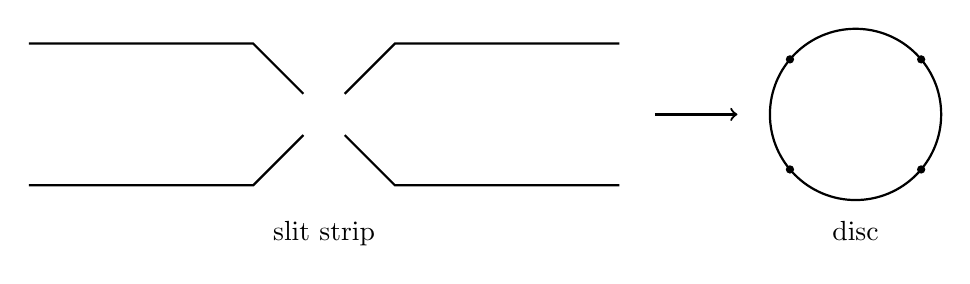
\begin{tikzpicture}[x=0.75cm,y=0.75cm]
    \draw[thick] (-5,1.2) -- (-1.2,1.2) -- (-0.35,0.35);
    \draw[thick] (-5,-1.2) -- (-1.2,-1.2) -- (-0.35,-0.35);
    \draw[thick] (0.35,0.35) -- (1.2,1.2) -- (5,1.2);
    \draw[thick] (0.35,-0.35) -- (1.2,-1.2) -- (5,-1.2);
    \draw[->,thick] (5.6,0) -- (7.0,0);
    \draw[thick] (9.0,0) circle (1.45);
    \foreach \a in {40,140,220,320} \fill (9.0,0) ++(\a:1.45) circle (1.5pt);
    \node[below] at (0,-1.65) {slit strip};
    \node[below] at (9.0,-1.65) {disc};
  \end{tikzpicture}
  \end{adjustbox}
  \caption{Сопоставление линий уровня на доске и наглядная схема
  конформного отображения полосы с разрезами на диск. Четыре внешних конца становятся
  четырьмя особыми граничными точками.}
  \lectureframe{01:04:46}
  \label{fig:l07-strip-to-disc}
\end{figure}

Внешние состояния при этой замене координат не теряются. Импульс,
тип частицы и уровень осциллятора должны быть вставлены в четырёх особых
точках. Формальные объекты, несущие эту информацию, — это вершинные операторы.
Их подробное построение откладывается, но их роль уже ясна:
они превращают иначе однородный интеграл по траекториям на мировой поверхности в конкретно
заданный процесс рассеяния.

После того как с помощью конформных преобразований диска три граничные
точки перенесены в удобные опорные положения, остаётся одна вещественная
относительная позиция. Её можно представить через двойное отношение четырёх упорядоченных
граничных точек. Это дисковый аналог прежнего времени жизни \(\tau_0\).

\begin{figure}[H]
  \centering
  \includegraphics[width=0.62\textwidth]{lecture_07_figure_13.png}
  \caption{Четыре точки вставки на границе диска. Конформная
  свобода устраняет все вещественные модули их упорядоченной конфигурации, кроме одного.}
  \lectureframe{01:10:55}
  \label{fig:l07-four-points}
\end{figure}

Следовательно, интеграл по времени жизни не исчез. Он превратился в
интеграл по этому оставшемуся модулю. Если выбрать стандартную координату
\(0<z<1\), четырёхточечный интеграл для открытой струны принимает тот же вид, что и в
предыдущей лекции,
\begin{equation}
  \mathcal A(s,t)\propto
  \int_0^1 z^{-s-1}(1-z)^{-t-1}\,dz.
  \label{eq:l07-modulus-integral}
\end{equation}

\section{Два предела одной поверхности}

В одном конце пространства модулей две точки вставки, соответствующие
входящей паре, сближаются. В координатах полосы с разрезами это
длинный интервал между соединением и расщеплением: промежуточная струна
прямого канала распространяется долго. На другом конце сближается другая соседняя
пара. Тогда ту же поверхность естественно интерпретировать как обмен в перекрёстном
канале. На полосе эти описания выглядят несвязанными, но являются соседними граничными пределами одного дискового интеграла.

Возвращаясь к соглашению предыдущей лекции о сигнатуре с преимущественно
положительными знаками,
\begin{equation}
  -s=(k_1+k_2)^2,
  \qquad
  -t=(k_1+k_3)^2.
  \label{eq:l07-mandelstam}
\end{equation}
В прямом пределе полюса организуются по \(s\); в перекрёстном пределе полюса
организуются по \(t\).
\editorialnote{Ближе к концу лекции на доске используется сокращённое соглашение
о знаках для инвариантов Мандельстама, и при этом \(s\) отождествляется с положительным
квадратом энергии в системе центра масс. Уравнение \eqref{eq:l07-mandelstam} сохраняет
соглашение с преимущественно положительной сигнатурой, установленное в лекции 6.}

\begin{figure}[H]
  \centering
  \includegraphics[width=0.62\textwidth]{lecture_07_figure_14.png}
  \caption{Две диаграммы каналов: длительное распространение в одной ориентации
  и обмен в перекрёстной ориентации.}
  \lectureframe{01:19:27}
  \label{fig:l07-channel-diagrams}
\end{figure}

\begin{figure}[H]
  \centering
  \includegraphics[width=0.72\textwidth]{lecture_07_figure_15.png}
  \caption{На доске вновь рассматриваются группировки импульсов в \(s\)- и \(t\)-каналах
  при сравнении двух пределов модуля диска.}
  \lectureframe{01:19:40}
  \label{fig:l07-st-board}
\end{figure}

Таким образом, один аналитический объект даёт оба разложения:
\begin{equation}
  \mathcal A(s,t)=\mathcal A(t,s).
\end{equation}
Это и есть дуальность каналов. В первоначальном языке резонансов казалось
чудом, что сумма по состояниям прямого канала может также кодировать обмен в перекрёстном
канале. На евклидовой мировой поверхности конформная симметрия объясняет,
почему оба описания относятся к одной и той же поверхности. Исторически
эта интерпретация появилась очень быстро после открытия амплитуды Венециано в 1969 году.

\begin{classroomqa}
\audiencequestion{Есть ли также представление в виде полосы с разрезами,
соответствующее перекрёстной ориентации? \lecturetimestamp{01:20:49}}
\lecturerresponse{Да, но направление, называемое временем, должно быть выбрано
иначе. Одну и ту же евклидову поверхность можно рассечь так, что другая пара
внешних концов окажется в далёком прошлом и будущем. Именно эта альтернативная
нарезка и объясняет, почему одна мировая поверхность допускает более одной
канальной интерпретации.}
\end{classroomqa}

\begin{classroomqa}
\audiencequestion{Определяется ли время, в течение которого струны остаются соединёнными,
константой связи? \lecturetimestamp{01:21:39}}
\lecturerresponse{Нет, никакое фиксированное время жизни не выбирается. Время жизни является
переменной интегрирования, и вклад даёт каждое значение. Константа связи управляет
весом соединения и расщепления --- эквивалентно, силой распада --- и
входит в амплитуду мультипликативно; она не заменяет интеграл по модулю.}
\end{classroomqa}